\documentclass[submit,techrep,noauthor]{ipsj}

\usepackage{amsmath,amssymb,amsfonts}
\usepackage{cite}
\usepackage[japanese]{babel}
\usepackage[scaled]{beramono}
\usepackage{booktabs}
\usepackage[T1]{fontenc}
\usepackage[dvipdfmx]{graphicx}
\usepackage[utf8]{inputenc}
\usepackage{listings}
\usepackage[all, warning]{onlyamsmath}
\usepackage{siunitx}
\usepackage[subrefformat=parens]{subcaption}
\usepackage{url}

\newcommand{\us}{\si{\micro\second}}

\begin{document}

\title{ベクトル型スーパーコンピュータ「AOBA-S」の性能評価}

\etitle{Performance Evaluation of a Vector Supercomputer ``AOBA-S''}

\affiliate{CSC}{東北大学サイバーサイエンスセンター}
\affiliate{NEC}{日本電気株式会社}
\affiliate{TU}{東北大学大学院情報科学研究科}
\affiliate{TDU}{東京電機大学}

\author{高橋 慧智}{Keichi Takahashi}{CSC,TU}[keichi@tohoku.ac.jp]
\author{藤本 壮也}{Soya Fujimoto}{NEC}[s-fujimoto@nec.com]
\author{長瀬 悟}{Satoru Nagarase}{NEC}[s.nagase@nec.com]
\author{磯部 洋子}{Yoko Isobe}{NEC}[y-isobe-pi@nec.com]
\author{下村 陽一}{Yoichi Shimomura}{CSC,TU}[shimomura32@tohoku.ac.jp]
\author{江川 隆輔}{Ryusuke Egawa}{TDU}[egawa@mail.dendai.ac.jp]
\author{滝沢 寛之}{Hiroyuki Takizawa}{CSC,TU}[takizawa@tohoku.ac.jp]

\begin{abstract}
東北大学サイバーサイエンスセンターは,2023年8月よりベクトル型スーパーコンピュータ「AOBA-S」の運用を
開始した.AOBA-Sは第3世代ベクトルエンジン (VE30) をノードあたり8基搭載した計504ノードから構成され,
理論演算性能は21.05\,PFLOP/s,メモリ帯域幅は9.97\,PB/sに達する世界最大規模のベクトル型
スーパーコンピュータである.本稿ではAOBA-Sの設計を概説し,運用開始に先駆けて実施したAOBA-Sの
初期性能評価の結果について報告する.
\end{abstract}

\begin{eabstract}
Cyberscience Center, Tohoku University has started the operation of a new vector supercomputer 
``AOBA-S'' in August 2023. AOBA-S comprises 504 compute nodes each equipped with eight
third-generation Vector Engine (VE30) cards. The peak compute performance and memory bandwidth of
AOBA-S reach 21.05\,PFLOP/s and 9.97\,PB/s, respectively, making it the world's largest vector
supercomputer as of writing this paper. In this paper, we describe the basic design of AOBA-S and
report the results of the initial performance evaluation that we have conducted prior to the
operation start of AOBA-S.
\end{eabstract}

\maketitle

\section{はじめに}

東北大学サイバーサイエンスセンター (以下本センター) では,1986年に高性能計算センターとして活動を
開始して以来,SX-1 (NEC製,0.57\,GFLOP/s) から一貫して,主力計算システムとして
ベクトル型スーパーコンピュータを導入し,最先端の学術研究を強力に支援,推進してきた.
本センターは全国の大学等の研究者が学術研究のために利用する全国共同利用施設であると同時に,
全国の情報基盤センター群と連携した学際大規模情報基盤共同利用・共同研究拠点 (JHPCN) の構成拠点である.
また,、「富岳」を中核とする全国の計算機資源を連携した革新的ハイパフォーマンス・コンピューティング・
インフラ (HPCI) の構成機関でもあ り、共同研究活動を推進する拠点となっている.

このような背景の下,本センターでは2020年10月にベクトル型スーパーコンピュータ「AOBA-A」および
スカラ型並列コンピュータ「AOBA-B」を導入し,高速で大規模な計算処理環境を提供している.
両サブシステムの利用率は常に高く,計算需要が処理能力を超える状況続いてきた.この
2022年10月にはクラウド上システムAOBA-Cによって計算能力の一時的な増強を実施したものの,
次期スーパーコンピュータ「AOBA-S」の構想・設計を進めてきた.AOBA-Sは2022年4月に入札公示を行い,
2022年8月に日本電気株式会社が落札し,2023年8月より利用者へのサービス提供を開始した.

AOBA-SはAOBA-Aに比較すると14倍以上のピーク演算性能と11倍以上のピークメモリ帯域幅を有し,
原稿執筆時点の2023年8月現在では,世界最高性能のベクトル型スーパーコンピュータである.
AOBA-Sの中核であるVector Engine Type 30AプロセッサはVector Engineプロセッサの第3世代であり,
第2世代に比べると演算性能やメモリ帯域幅等の基本性能の向上に加え,大幅にアーキテクチャが改善されている.
そのため,ピーク演算性能やピークメモリ帯域幅の向上以上にアプリケーションの性能向上が期待できるため,
運用に先駆けて各種性能評価を実施した.本稿では,性能評価の結果について報告する.

\section{スーパーコンピュータ「AOBA-S」}

\subsection{概要}

AOBA-Sは,504ノードのNEC製SX-Aurorao TSUBASA C401-8から構成されるスーパーコンピュータである.

\begin{figure}
  \centering
  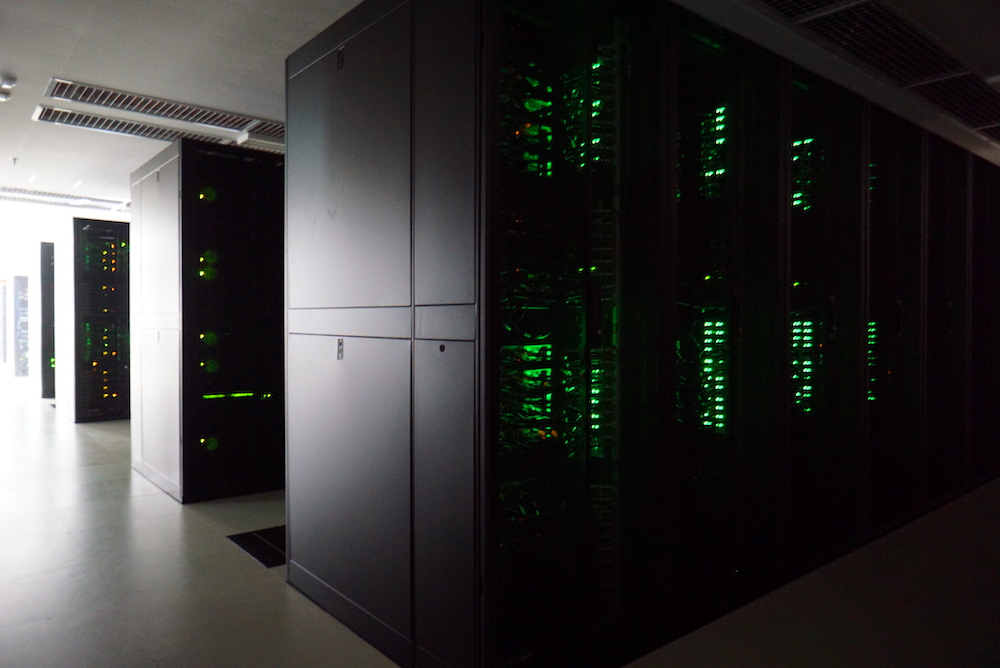
\includegraphics[width=.9\columnwidth]{figs/rack.jpg}
  \caption{AOBA-Sの外観}\label{fig:aoba-s}
\end{figure}

\subsection{SX-Aurora TSUBASA C401-8}

図\ref{fig:node}にAOBA-Sを構成するSX-Aurora TSUBASA (SX-AT) C401-8ノードの概念図を示す.
SX-Aurora TSUBASAはVector Host (VH) とVector Engine (VE) の2種のプロセッサが搭載した
ヘテロジニアスな計算機である.VEはPCI Expressカード上に実装されたベクトルプロセッサであり,HBMと
密結合されたことにより.VHはVEから発行されたI/O等のOS処理を担うためのx86\_64プロセッサである.
SX-AT C401-8はVHとして64コアのAMD EPYC 7763 CPUを採用しており,各ノードに8基のVector Engine Type
30Aカードを搭載している.8基のVEは2基ずつ共有するPCIeスイッチを経由し,VHに接続している.
VEは1基あたり96\,GBのHBM2Eメモリ,VHは256\,GBのDDR4メモリを搭載している.また,VHには2基のInfiniBand
NDR 200G HCAが搭載されており,VHおよびVE間の通信手段として利用することが可能である.

\begin{figure}
  \centering
  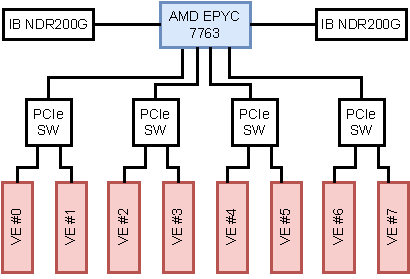
\includegraphics{figs/node_arch.pdf}
  \caption{SX-Aurora TSUBASA C401-8の構成}\label{fig:node}
\end{figure}

\begin{figure}
  \centering
  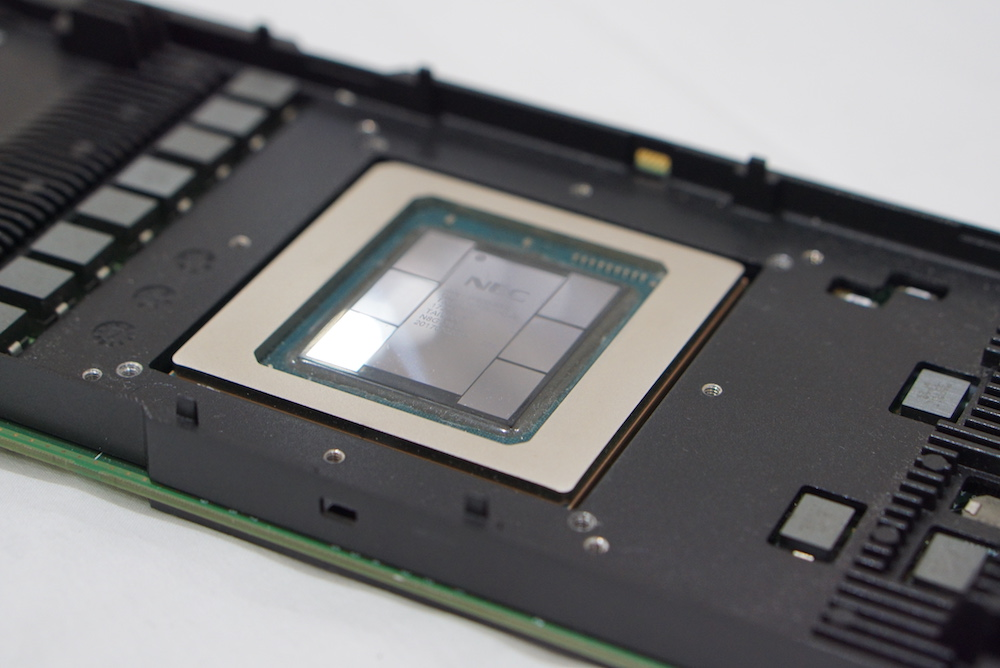
\includegraphics[width=.9\columnwidth]{figs/ve30.jpg}
  \caption{Vector Engine Type 30Aの外観}\label{fig:ve-card}
\end{figure}

図\ref{fig:ve30}にVector Engine Type 30A (VE30)プロセッサの概要を示す.VE30はVector
Engineプロセッサの第3世代となるプロセッサである.VE30は16個のベクトルコアを搭載し,これらの
ベクトルコアが2次元メッシュ型Network on Chip (NoC)によって接続されている.
ベクトルコア群はNoCによって6.4\,TB/sの帯域幅を有するLast Level Cache 
(LLC) に接続しており,さらにLLCは2.45\,TB/sの帯域幅を有する96\,GBのHBM2Eメモリに接続している.
各ベクトルコアはScalar Processing Unit (SPU) とVector Processing Unit (VPU) という2種の実行ユニット
を搭載している.SPUは命令をフェッチ,デコードし,VPUへベクトル命令を発行する.VPUはベクトル命令を
実行する.SPUにはL1キャッシュとL2キャッシュが搭載されており,さらに,VE30ではSPUとVPUが共有する
2\,MBのL3キャッシュが追加されている.

\begin{figure}
  \centering
  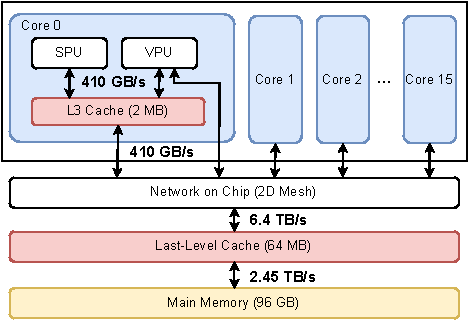
\includegraphics{figs/ve30_memory_hierarchy.pdf}
  \caption{VE30の概要図~\cite{Takahashi2023}}\label{fig:ve30}
\end{figure}

前世代のVE Type 20Aと比較すると,ベクトルコアあたりの計算性能とメモリアクセス性能を同一である一方,
コア数が10コアから16コアへ1.6倍に増加している.また,コア数の増加に応じてメモリ帯域幅も1.53\,TB/sから
2.54\,TB/sへ1.6倍に向上している.さらに,メモリ容量は48\,GBから96\,GBへ2倍に拡大され,LLCの容量は
16\,MBから64\,MBへ4倍に拡大している.

\subsection{AOBA-S}

\begin{table}
\centering
\caption{AOBA-Sの性能諸元}\label{tbl:aoba-s}
\begin{tabular}{@{}lll@{}}
\toprule
ノード数        & ノード単体     & システム全体           \\ \midrule
VE数            & 8              & 4,032                  \\ \midrule
VH数            & 1              & 504                    \\
VE理論演算性能  & 39.28\,TFLOP/s & 19.79\,PFLOP/s         \\
VEメモリ帯域幅  & 19.60\,TB/s    & 9.87\,PB/s             \\
VEメモリ容量    & 768\,GB        & 378\,TB                \\ \midrule
VH理論演算性能  & 2.50\,TFLOP/s  & 1.26\,PFLOPS/s         \\
VHメモリ帯域幅  & 0.20\,TB/s     & 0.1\,PB/s              \\
VHメモリ容量    & 256\,GB        & 126\,TB                \\ \midrule
相互結合網      & \multicolumn{2}{c}{InfiniBand NDR}      \\
共有ストレージ  & \multicolumn{2}{c}{Lustre 4.4\,PB}      \\ \bottomrule
\end{tabular}
\end{table}

AOBA-Sは,504ノードのSX-Aurorao TSUBASA C401-8から構成されるスーパーコンピュータである.
物理的には1ラックに16 VHが搭載されており,32ラックに計504 VHが収容されている.
これに加え,フロントエンドサーバ群および管理・監視サーバに2ラック,ネットワーク機器が2ラック,
UPSが3ラック,ストレージが1ラックの計8ラックに収容されている.

相互結合網にはInfiniBand NDRを採用しており,図\ref{fig:topo}に示すように,
フルバイセクション帯域幅およびノンブロッキングの2段Fat-treeトポロジによって計算ノード,
ストレージノード,およびフロントエンドノードが接続されている.相互結合網は16基のスパインスイッチおよび
18基のリーフスイッチによって構成される.リーフスイッチのうち16基には計算ノードが接続されており,
残りの2基にはストレージおよびフロントエンドノードが接続されている.計算ノードが接続されている
各リーフスイッチには32 VH (64 HCA) が接続されている.スパインスイッチとリーフスイッチの間は2本の
400\,Gbpsリンクによって接続されており,計算ノード部分のバイセクション帯域幅は204.8\,Tbpsに達する.

\begin{figure}
  \centering
  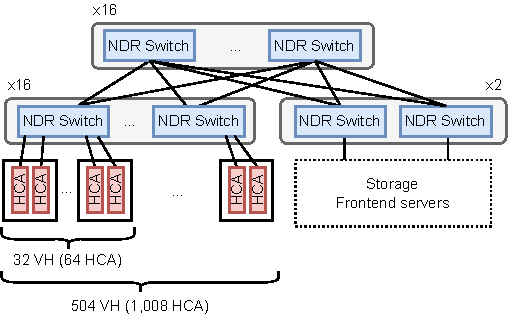
\includegraphics{figs/nw_topology.pdf}
  \caption{AOBA-S相互結合網のトポロジ}\label{fig:topo}
\end{figure}

ストレージにはDDN社製ES400NVX2アプライアンスを採用している.
1基のES400NVX2がLustre MDS/MDTとして動作し,もう1基のES400NVX2がOSS/OSTとして動作する.
OSS/OST用ES400NVX2には4基のSS9012エンクロージャが接続され,合計332本の7200\,rpm NL-SAS
HDDを搭載している.各ES400NVX2は8本のInfiniBand HDRリンクによって相互結合網に接続している.

\section{性能評価結果}

本節では,

\subsection{プロセッサ単体性能}

本節では,業界標準のベンチマークであるBabelStream~\cite{Deakin2018},
High Performance Linpack (HPL)~\cite{Dongarra2003},およびHigh Performance Conjugate
Gradients (HPCG)~\cite{Dongarra2016}を用いてVE30プロセッサの単体性能を同世代の他プロセッサと比較する.
比較対象のプロセッサは,前世代のVEであるVE Type 20B,富士通A64FX,Intel Xeon Platinum 8368
(IceLake),NVIDIA A100 40\,GBおよび80\,GBモデルである.HPLおよびHPCGのバイナリには,
各プロセッサのベンダより提供されている最適化されたバイナリを使用した.なおA64FXについてはバイナリを
入手できなかったため,Top500に掲載されている全系実行の性能より推定した.各プロセッサの諸元については,
文献~\cite{Takahashi2023}を参照されたい.

\subsubsection{基本性能}

図\ref{fig:stream}にBabelStream v4.0によって計測した各プロセッサの実効メモリ帯域幅を示す.
VE30の実効メモリ帯域幅は1.79\,TB/sとなり,他のすべてのプロセッサより高い性能となった.
一方,ピークメモリ帯域幅に対する効率は72\%であり,これはA100 40\,GBモデルの91\%や80\,GBモデルの
86\%に比べると低い.これは,VEのキャッシュラインサイズが128\,Bであるのに対し,GPUの
キャッシュラインサイズが256\,Bと2倍の大きさであるため,STREAMのように粒度の粗い連続アクセスにおいて
GPUが有利であることに起因している可能性がある.

\begin{figure}
  \centering
  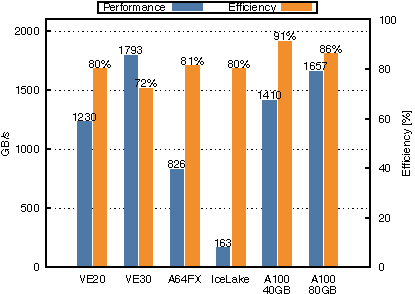
\includegraphics{figs/stream.pdf}
  \caption{BabelStream性能~\cite{Takahashi2023}}\label{fig:stream}
\end{figure}

図\ref{fig:hpl}にHPLベンチマークの性能を示す.HPLは演算律速なベンチマークであるため,ピーク演算性能が
高いA100 40\,GBモデルと80\,GBモデルの実効性能が11.8\,TFLOP/sと12.5\,TFLOP/sと非常に高い.
一方,実行効率は60\%台とVEやA64FXに比べると低い.
実行中に\verb|nvidia-smi|コマンドでGPUの周波数を監視すると周波数が低下しており,
PCIe版では電力供給が不足し,パワースロットリングによって性能低下していると考えられる.
VE30の性能は4.43\,TFLOP/sとなり,A100の両モデルに次いで最も高くなった.実行効率は90\%であり,実行中に
\verb|vecmd|コマンドで周波数を監視したところ,パワースロットリングは発生していなかった.

\begin{figure}
  \centering
  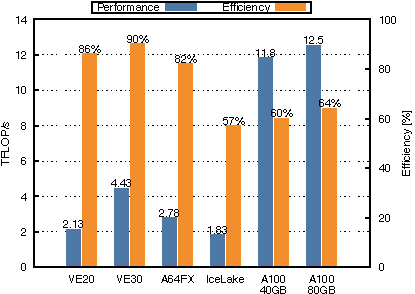
\includegraphics{figs/hpl.pdf}
  \caption{HPL性能~\cite{Takahashi2023}}\label{fig:hpl}
\end{figure}

図\ref{fig:hpcg}にHPCGベンチマークの性能を示す.VE30におけるHPCGベンチマークの性能は258\,GFLOP/sであり,
A100 80\,GBモデルの259\,GFLOP/sとほぼ同等の結果となった.実行効率は5.2\%であり,A100 80\,GBモデルの
2倍となった.

\begin{figure}
  \centering
  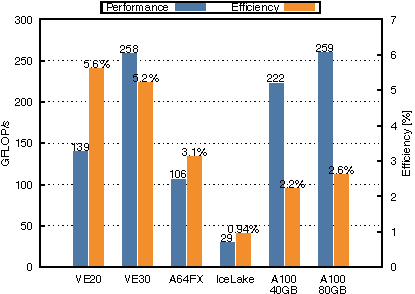
\includegraphics{figs/hpcg.pdf}
  \caption{HPCG性能~\cite{Takahashi2023}}\label{fig:hpcg}
\end{figure}

\subsubsection{東北大カーネル集}

実アプリケーションにおける性能を計測するため,本センターの利用者が開発した
アプリケーションから抽出したカーネルのカタログである東北大カーネル集の性能を測定した.
東北大カーネル集は,表\ref{tbl:isc-kernels}に示す6つのカーネルからなる.それぞれのカーネルは表に示す通り,
それぞれ律速要因が異なる.

\begin{table}
\caption{東北大カーネル集}\label{tbl:isc-kernels}
\begin{tabular}{@{}lll@{}}
\toprule
カーネル名                          & 科学分野        & 律速要因            \\ \midrule
Earthquake~\cite{Ariyoshi2007}      & 地震学          & メモリ帯域幅        \\
Turbulent Flow~\cite{Tsukahara2007} & 流体力学        & LLC帯域幅           \\
Antenna~\cite{Sato2011}             & 電波工学        & メモリ帯域幅        \\
Land Mine~\cite{Sato2003}           & 電波工学        & メモリ帯域幅        \\
Turbine~\cite{Tsukahara2007}        & 流体力学        & メモリレイテンシ    \\
Plasma~\cite{Katoh2005}             & プラズマ科学    & メモリレイテンシ    \\ \bottomrule
\end{tabular}
\end{table}

図\ref{fig:isc-kernels}にVE20およびVE30における東北大カーネル集の性能を示す.VE30では,新設された
L3キャッシュの効果を明らかにするため,L3キャッシュをバイパスした際の性能も合わせて示している.

\begin{figure}
  \centering
  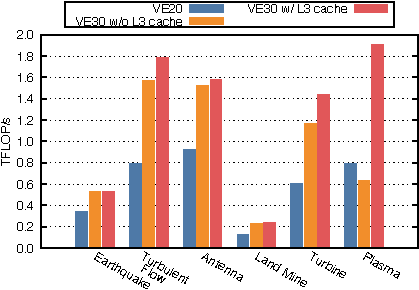
\includegraphics{figs/isc_kernels.pdf}
  \caption{東北大カーネル集の性能}\label{fig:isc-kernels}
\end{figure}

\subsection{HPL・HPCG性能}

High Performance Linpack (HPL)~\cite{Dongarra2003}ベンチマークおよびHigh Performance Conjugate
Gradients (HPCG)~\cite{Dongarra2016} ベンチマークを実行した.
504 VHの全系実行では,HPLの性能が16.33\,PFLOP/s (実行効率82.4\%),HPCG性能が913.1\,TFLOP/s 
(実行効率4.61\%) なお,これらの性能はパラメータのチューニング等の最適化を実施する前の性能であり,
今後チューニングを実施することにより,さらに性能が向上する予定である.

\begin{figure}
  \centering
  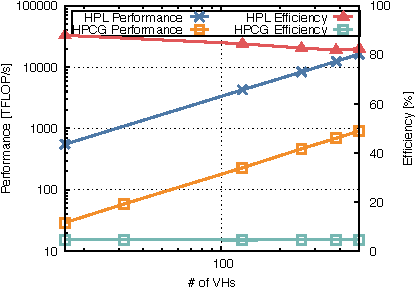
\includegraphics{figs/hpl_hpcg.pdf}
  \caption{HPLおよびHPCG性能}\label{fig:hpl-hpcg}
\end{figure}

\subsection{MPI通信性能}

OSU Micro-Benchmarks
7.2\footnote{\url{https://mvapich.cse.ohio-state.edu/benchmarks/}}を用いてMPI通信の性能を計測した.
NCC 5.0.1でコンパイルし,MPIライブラリにNEC MPI 3.4.0を用いた.
測定にあたっては,(1) 同一PCIeスイッチに接続されたVE間,(2)
同一ノード内の異なるPCIeスイッチに接続されたVE間,(3) 同一ラックの異なるノードに接続されたVE間,
の3パターンを計測した.

\subsubsection{1対1通信}

図\ref{fig:mpi-lat}に\verb|osu_latency|ベンチマークで計測したMPI 1対1通信のレイテンシを示す.
\verb|-i 1000 -x 500|
同一ノード内の同一PCIeスイッチに接続されたVE間の最低レイテンシは1.51\us であった.
同一ノード内の別PCIeスイッチに接続されたVE間ではルートコンプレックスを経由する必要があり,
レイテンシは1.88\us であった.
ノード間 3.87\us
ノード間 2.09\us

\begin{figure}
  \centering
  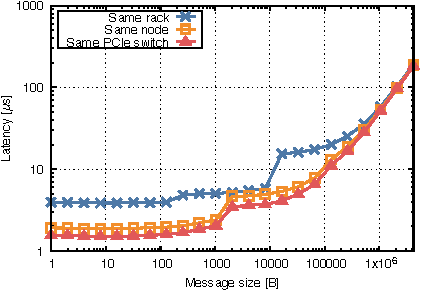
\includegraphics{figs/mpi_latency.pdf}
  \caption{MPI 1対1通信のレイテンシ}\label{fig:mpi-lat}
\end{figure}

図\ref{fig:mpi-lat}に\verb|osu_bandwidth|ベンチマークで計測したMPI 1対1通信のスループットを示す.

PCIe Gen 4 $\times$16の実効帯域幅31.508\,GB/sである.73.4\%

\begin{figure}
  \centering
  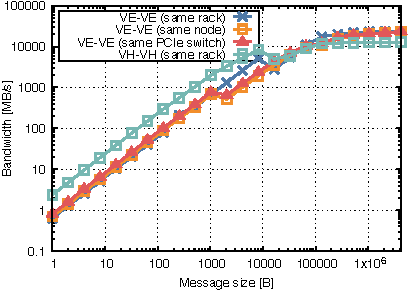
\includegraphics{figs/mpi_bandwidth.pdf}
  \caption{MPI 1対1通信のスループット}\label{fig:bw}
\end{figure}

\subsubsection{集団通信}

\subsection{ストレージ性能}

IOR 3.3.0\footnote{\url{https://github.com/hpc/ior}}を用いて並列ファイルシステムのスループットを計測した.
1VEにつきIORを1プロセスを起動し,1プロセスあたり1ファイルに書き込む設定で計測を実施した.

計測に用いたコマンドは,
\texttt{ior -w -r -a POSIX -F -Q 8 -C -e -g -b 16m -t 4m -s 250 -i 3}である.
書き込み時のページキャッシュの効果を排除するため,\texttt{-e}オプションによってwrite完了時に
\texttt{fsync()}を呼び出している.また,読み込み時のページキャッシュの効果を排除するため,書き込み
プロセスと読み込みプロセスをずらす\texttt{-C}オプションを指定している.また,同一VHに接続された
VEはVH側においてページキャッシュを共有するため,書き込みVEと読み込みVEがそれぞれ異なるVHに所属する
ように\texttt{-Q 8}オプションによって書き込みと読み込みプロセスを8ランク分ずらしている.

図\ref{fig:ior}に計測結果を示す.1024 VEにおいて書き込み49.2\,GB/s,読み込み39.0\,GB/sのスループット
を達成した.

\begin{figure}
  \centering
  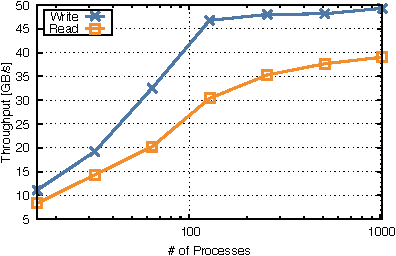
\includegraphics{figs/ior.pdf}
  \caption{並列ファイルシステムのスループット}\label{fig:ior}
\end{figure}

\subsection{SPEChpc}

SPEChpc 1.1.7

\subsubsection{Tinyサイズ}

\subsubsection{Largeサイズ}

Largeサイズの実行結果はSPEC公式サイトでも未だ限られているので
\footnote{\url{https://www.spec.org/hpc2021/results/}},ここでは文献~\cite{Brunst2022}において計測が
なされた,独J\"{u}lich Supercomputing Centreが運用するJUWELS Booster上での性能測定結果と比較する.
JUWELS BoosterはAMD EPYC 7402を2ソケットとNVIDIA A100 SXM4
40\,GBを4基搭載した計算ノード936台から構成される.相互結合網にはDragonFly+トポロジを採用し,ノード
あたりInfiniBand HDR200を4ポート備える.

図\ref{fig:spechpc-profile}に各ベンチマークの実行時間に占めるMPI通信時間を示す.なお,
本プロファイラを利用するには,\verb|-mpiprof|コンパイラオプションを用いて
実行時に\verb|NMPI_PROGINF|環境変数に\verb|YES|を設定する.

NEC MPI\footnote{\url{https://sxauroratsubasa.sakura.ne.jp/documents/mpi/pdfs/g2am01-NEC_MPI_User_Guide_ja.pdf}}

BoosterではNVLink 3.0によってノード内のGPUが全結合されており,GPU間のリンク帯域幅は片方向200\,GB/s
である.一方,AOBA-SではVE間はルートコンプレックスを根とするツリー型トポロジで接続されており,
リンク帯域幅は30.5\,GB/sである.したがって,Boosterのノード内バイセクション帯域幅は800\,GB/sである
一方,AOBA-Sは30.5\,GB/sと,26倍以上の差がある.
また,Boosterではノード間接続の帯域幅はノードあたり800\,Gbpsであるが,AOBA-Sでは400\,Gbpsであり,
2倍の差がある.これらの理由により,BoosterではMPI通信時間が短いと推測される.

\begin{figure}
  \centering
  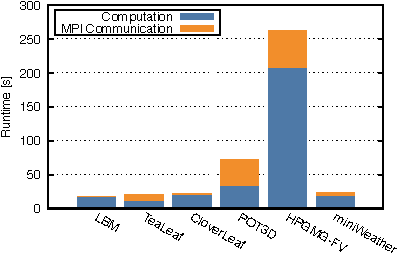
\includegraphics{figs/spechpc_profile.pdf}
  \caption{SPEChpc Largeサイズの実行時間内訳}\label{fig:spechpc-profile}
\end{figure}

\section{おわりに}

\subsection*{謝辞}

性能評価にご協力いただいた東北大学情報部デジタルサービス支援課および日本電気株式会社の皆様に
感謝いたします.

\bibliographystyle{IEEEtran}
\bibliography{references}

\end{document}
